\documentclass[a4paper]{article}

%% Language and font encodings
\usepackage[english]{babel}
\usepackage[utf8x]{inputenc}
\usepackage[T1]{fontenc}

%% Sets page size and margins
\usepackage[a4paper,top=3cm,bottom=2cm,left=3cm,right=3cm,marginparwidth=1.75cm]{geometry}

% packages
\usepackage{tikz}
\usepackage{amsmath, amsfonts}
\usepackage{graphicx}
\usepackage[colorinlistoftodos]{todonotes}
\usepackage[colorlinks=true, allcolors=blue]{hyperref}
\usetikzlibrary{matrix,fit}

% commands
\newcommand{\tikzmark}[2]{
    \tikz[overlay,remember picture,baseline] 
    \node[anchor=base] (#1) {$#2$};
}

\tikzset{
  highlight/.style={triangle,rounded corners,fill=red!15,draw,fill opacity=0.5,thick,inner sep=0pt}
}

\newenvironment{sbmatrix}[1]
 {\def\mysubscript{#1}\mathop\bgroup\begin{bmatrix}}
 {\end{bmatrix}\egroup_{\textstyle\mathstrut\mysubscript}}
 
\pgfdeclarelayer{background}
\pgfsetlayers{background,main}

\title{Stats Learning Lecture Week 1}

\begin{document}

\section{Notes}
  \subsection{Matrix Object Intro}
  You're probably used to seeing data in a spreadsheet looking something like this:

    $$\begin{matrix}
    & \text{Race} & \text{Class} & \cdots & \text{Age}\\
    \text{Garrett} & \text{human} & \text{warrior} & \cdots & 27\\
    \text{Varric} & \text{dwarf} & \text{rogue} & \cdots & 30\\
    \vdots & \vdots & \vdots & \ddots & \vdots \\
    \text{Merrill} & \text{elf} & \text{mage} & \cdots & 22
    \end{matrix}$$

  Where each row represents one individual, or one observation, and the columns reflect attributes about these observations. In the above scenario, data on the character from a video game called Dragon Age:2 are recorded so that each character represents a row and their attributes (like their race, their fighting class, and their age) make up each of the columns.

  While spreadsheets are helpful in storing and looking at data, data is put into matrices to perform analyses and for modeling. A matrix is a rectangular representation of data where rows represent observations and columns represent attributes.

  Now let's transform our spreadsheet into a matrix object. As a matrix, it would look similar but now with only the observations inside:

    $$\begin{bmatrix}
    \text{human} & \text{warrior} & \cdots & 27\\
    \text{dwarf} & \text{rogue} & \cdots & 30\\
    \vdots & \vdots & \ddots & \vdots \\
    \text{elf} & \text{mage} & \cdots & 22
    \end{bmatrix}$$

  A generic view of the spreadsheet can be visualized below to give you a better idea of how numbering works in matrices across rows and columns.

    $$\begin{matrix}
    & x_1 & x_2 & \cdots & x_p\\
    \text{individual } 1 & x_{11} & x_{12} & \cdots & x_{1p}\\
    \text{individual } 2 & x_{21} & x_{22} & \cdots & x_{2p}\\
    \vdots & \vdots & \vdots &\ddots & \vdots \\
    \text{individual } i & x_{i1} & x_{i2} & \cdots & x_{ip}\\
    \vdots & \vdots & \vdots & \ddots & \vdots \\
    \text{individual } n & x_{n1} & x_{n2} & \cdots & x_{np}
    \end{matrix}$$

Now converting our generic spreadsheet to a generic matrix, we say that matrix $X$ is equal to:
   $$\begin{bmatrix}
     x_{11} & x_{12} & \cdots & x_{1p}\\
    \vdots & \vdots & \ddots& \vdots \\
     x_{i1} & \cdots & \cdots & x_{ip}\\
    \vdots & \vdots & \ddots & \vdots \\
     x_{n1} & \cdots & \cdots & x_{np}
    \end{bmatrix}$$

    $$X\equiv (x_{ij, i=1,...,n, j=1,...,p})$$
  Here $X$ is a data matrix that has n observations and p variables (attributes).

If the number of columns,$p$, in a matrix equals the number of rows, $n$, in a matrix, then that matrix is called a square matrix since the shape is that of a square. For example, below is a square matrix where $p=3$ and $n=3$:

   $$\begin{bmatrix}
    1 & 3 & 2 \\
    7 & 4 & 1\\
    4 & 6 & 7
    \end{bmatrix}$$

  There are four basic types of data that each column ($x_{j}$) can be:

  \begin{enumerate}
      \item $x_{j} \in \mathbb{R}$
      \newline \indent For example, data such as BMI and blood pressure would be placed here.

      \item $x_{j} \in {0,1}$
      \newline \indent For example, this would mean the data could follow a Bernoulli distribution like if the variable were gender; 0 could be coded for girl and 1 for boy. 

      \item $x_{j} \in \mathbb{N}$
      \newline \indent This would be for categorical data mainly, like the surveys that ask you how pleased you were with their service on a scale of 1 to 5. You could also transform the first spreadsheet into this type of data where numbers now represent certain values. For example, the Race column can be translated to show $1$ for human, $2$ for dwarf, and $3$ for elf. This would be considered factor data in R.

      \item $x_{j}$ is written words
      \newline \indent This would be for categorical data where information is filled like an open response question. We will not be handling such data in this class since it requires text mining.
  \end{enumerate}

    $\bf{X}$ is called a data matrix when $$\bf{X}=(\bf{x_{ij}}), i=1, ... , n , j=1, ... ,p$$

    where $\bf{x_i}$ is the vector of attributes of the $i^{th}$ is:

    $\bf{x_{i}}=(x_{i1}, x_{i2}, ... , x_{ip})^T= \begin{pmatrix}x_{i1}\\ x_{i2}\\\vdots\\x_{ip} \end{pmatrix}$

  Sometimes you may get data where variables are not all in the same scale, in these cases it is prudent to standardize the data in some way (whether that be cubitizing, unitizing, etc.) These topics will be explored further later on in the class, but are important to keep in mind when looking at any data.

An identity matrix is one that when added to another does not change the values at all. Mathematically this can be shown as:
	\begin{align*}
    A \times I &= A \\
    I \times A &= A
    \end{align*}
 As a rule of thumb, the identity matrix is a square matrix that looks like:    
       $$I =\begin{bmatrix}
     1 & 0 & \cdots & 0\\
     0 & 1 & \cdots  & 0\\
     \vdots & \vdots & \ddots & \vdots \\
     0 & 0 & \cdots &1
    \end{bmatrix}$$
    
    Notice how only some values are 1? This matrix is also called a diagonal matrix since there are 0s everywhere except the main diagonal which is all 1s. 
     \begin{equation}
        \begin{bmatrix}
          \tikzmark{top}{1} & 0 & 5	& 4 \\
             3 & 1 & 4 & 0\\
             2 & 5 & 5 & 7 \\
             0 & 0 & 8 & \tikzmark{bottom}{1}
        \end{bmatrix}
      \end{equation}

     \begin{tikzpicture}[overlay,remember picture]
         \draw[yellow, opacity=.4,line width=3mm,line cap=round] (top.center) -- (bottom.center);
    \end{tikzpicture}

    In general, the diagonal of a matrix always refers to the items along the main diagonal. The diagonal of a 4 X 4 matrix is highlighted below. Of note, in matrix algebra, the diagonal function always returns the main diagonal of a matrix in a matrix where every other item is 0s. This differs from R's \textit{diag} function which will only return the diagonal of the matrix as a vector. Another aspect in square matrices to be aware of is the upper and lower triangle. The upper triangle refers to all data points above and including the diagonal whereas the lower triangle refers to all data points below and including the diagonal.
 
\begin{center}
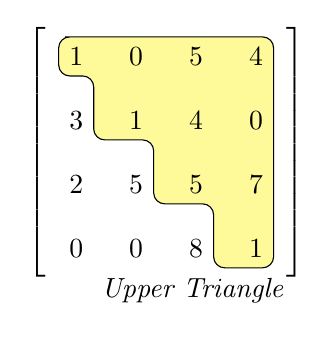
\begin{tikzpicture}[scale=3,line width=1pt]
 \matrix[matrix of math nodes,left delimiter={[},right delimiter={]},row sep=10pt,column sep = 10pt] (m)
    {
            1 & 0 & 5	& 4 \\
            3 & 1 & 4 & 0\\
            2 & 5 & 5 & 7 \\
            0 & 0 & 8 & 1\\
    };
\begin{pgfonlayer}{background}
      \node[inner sep=3pt,fit=(m-1-1)]          (1)   {};
      \node[inner sep=3pt,fit=(m-1-2) (m-2-4)]  (2)   {};
      \node[inner sep=3pt,fit=(m-3-3) (m-3-4)]  (3)   {};
      \node[inner sep=3pt,fit=(m-4-4)]          (4)   {};
 \draw[rounded corners,solid,fill=yellow,inner sep=3pt,fill opacity=0.4]
 (m-1-1.west) |- (m-1-1.south east) |- (m-2-2.south east) |- (m-3-3.south east) |- (m-4-4.south east) |- (m-1-1.north) -| (m-1-1.west);
\end{pgfonlayer}
\node at (0.5,-0.2,1) {\textit{Upper Triangle}};
\end{tikzpicture}
\hspace{1cm}
  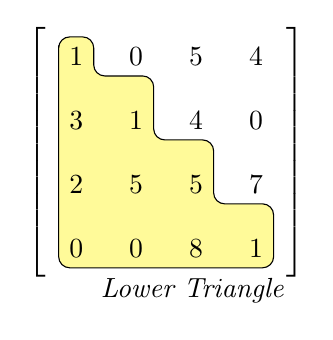
\begin{tikzpicture}[scale=3,line width=1pt]
    \matrix[matrix of math nodes,left delimiter={[},right delimiter={]},row sep=10pt,column sep = 10pt] (m)
    {
            1 & 0 & 5	& 4 \\
            3 & 1 & 4 & 0\\
            2 & 5 & 5 & 7 \\
            0 & 0 & 8 & 1\\
    };
    \begin{pgfonlayer}{background}
      \node[inner sep=3pt,fit=(m-1-1)]          (1)   {};
      \node[inner sep=3pt,fit=(m-2-1) (m-4-2)]  (2)   {};
      \node[inner sep=3pt,fit=(m-3-3) (m-4-3)]  (3)   {};
      \node[inner sep=3pt,fit=(m-4-4)]          (4)   {};
      \draw[rounded corners,solid,fill=yellow,inner sep=3pt,fill opacity=0.4]
      (m-1-1.north) -| (m-1-1.south east) -| (m-2-2.south east) -| (m-3-3.south east) -| (m-4-4.south east) -| (m-1-1.west)|- (m-1-1.north);
    \end{pgfonlayer}
    \node at (0.5,-0.2,1) {\textit{Lower Triangle}};
  \end{tikzpicture}
\end{center}


There is another special type of matrix to be aware of: those with either 1 row or 1 column. These are actually vectors.

\begin{equation*}
 \begin{sbmatrix}{1\hspace{2pt}Column}
    1\\
    0\\
    4\\
    6
  \end{sbmatrix}
  \begin{sbmatrix}{1\hspace{2pt}Row}
    1 & 0 & 4 & 6
  \end{sbmatrix}
\end{equation*}
\textbf{\textit{((Correlation matrix example for video!))}}

    
  \subsection{Vector Math}


The norm of a vector, written as $||x||$, gives the magnitude, or size, of a vector. There are different kinds of norms to be aware of, but in general the L1 and L2 norm are the most important.

Given a vector, $x=(x_1,x_2,\dots,x_n)$, the L1 ($||x||_1$)  and L2 ($||x||_2$) norm are defined as:

\begin{align*}
||x||_1 &= |x_1| +|x_2| +\dots + |x_n|\\
||x||_2 &= \sqrt{x_1^2 +x_2^2 +\dots + x_n^2}
\end{align*}

These norms often define the loss functions that models use when determining fit.

In a similar vein, the inner product, also known as the dot product, of 2 vectors is a function that produces a single number. For 2 vectors $a=(a_1,a_2,\dots,a_n)$ and $b=(b_1,b_2,\dots,b_n)$, we calculate the dot product as: $$\sum_{i=1}^{n}a_{1}b_{1}+a_{2}b_{2}+\cdots+a_{n}b_{n}$$

\textbf{\textit{In homework have students calculate dot product of 2 orthogonal vectors. Have AIO pop up video explaining importance of orthogonal vectors. Show that in real data set, if 2 attributes are orthogonal then they explain entirely different aspects about the data that do not overlap/are not correlated in any way.}}


    
  \subsection{Matrix Arithmetic}
  
Matrices can only be added or subtracted from one another if they are of the same dimensions. For example:
\begin{tabular}{ccc}
  $x=\begin{bmatrix}
    x_1\\
    x_2\\
    \vdots\\
    x_p
  \end{bmatrix}$ &
  $y=\begin{bmatrix}
    y_1\\
    y_2\\
    \vdots\\
    y_p
  \end{bmatrix}$ &
  $x+y=\begin{bmatrix}
    x_1+y_1\\
    x_2+y_1\\
    \vdots\\
    x_p+y_p
  \end{bmatrix}$
\end{tabular}

Multiplying a scalar with a matrix simply means that the scalar is distributed to every item of the matrix. For example:

\begin{tabular}{c}
  $cx=c\begin{bmatrix}
    x_{11} & x_{12} & x_{13}\\
    x_{21} & x_{22} & x_{23}
  \end{bmatrix}$
  $=\begin{bmatrix}
    cx_{11} & cx_{12} & cx_{13}\\
    cx_{21} & cx_{22} & cx_{23}
  \end{bmatrix}$
\end{tabular}

When multiplying matrices there's a few rules to follow:

\begin{itemize}
\item \textbf{You can only multiply if the number of columns in the first item equals the number of rows in the second item.} Thus if matrix $A$ is $n\times p$, then matrix $B$ must be $p\times m$. For the below example we're multiplying a $(1\times2)$ matrix by a $(2\times2)$ matrix.
\item \textbf{The outcome of multiplying two matrices $A$, which is $n\times p$, and  $B$, which is$p\times m$, will always be $C$, a  $n\times m$ matrix.} For the below example, this means our otcome of multiplying a $(1\times2)$ matrix by a $(2\times2)$ matrix should be a $1\times 2$ matrix.
\item \textbf{To multiply matrices, we compute the dot product of each row in matrix A with every column in matrix B.} Thus for our example, we start with row 1 of matrix A and column 1 of matrix B. Then move to row 1 of matrix A with column 2 of matrix B.
\end{itemize}

\begin{align*}
  \begin{bmatrix}
    x_1 & x_2
  \end{bmatrix}
  \begin{bmatrix}
    a & b\\
    c & d
  \end{bmatrix} &= \begin{bmatrix}
    ax_1+cx_2 & bx_1+dx_2
  \end{bmatrix}\\
  &= ax_1^2+cx_1x_2+bx_1x_2+dx_2^2
\end{align*}

The transpose of a vector simply flips the vector such that a vertical vector becomes horizontal and a horizontal vector becomes vertical:
\begin{center}
\begin{tabular}{c}
$a = \begin{bmatrix}
      2 & 3 & -1
      \end{bmatrix}$
$a^T = \begin{bmatrix}
        2\\
        3 \\
        -1
        \end{bmatrix}$
\end{tabular}
\end{center}
Similarly a transposed matrix is a flipped version of itself. To find the transpose, you can first find the diagonal of the matrix and then switch the row and column indices of the non diagonal objects.
\begin{center}
\begin{tabular}{c}
 $A = \begin{bmatrix}
       0 & 1 & 3\\
       -a_1 & -a_2 & 0
       \end{bmatrix}$
 $ A^T = \begin{bmatrix}
         0 & -a_1\\
         1 & -a_2\\
         3 & 0
         \end{bmatrix}$
 \end{tabular}               
\end{center}

\textbf{\textit{Above would be best in a GIF like on the wiki page for transpose!}}

A square matrix, $A$, is invertible (has an inverse) if a matrix, $A^{-1}$ exists that when multiplied with $A$ the identity matrix is produced
\begin{center}
\begin{align*}
 A \times A^{-1} &= I\\
 A^{-1} \times A &= I
 \end{align*}
\end{center}

Be careful here! not every square matrix has an inverse; in order to determine if one exists, you'll have to know a bit more about matrices.
    
  \subsection{Harder Matrix Math}

Sometimes it may be useful to break up a matrix into smaller chunks, this is called partitioning. 

For example, let
$$A = \begin{bmatrix}
    x_{11} & x_{12} & x_{13}\\
    x_{21} & x_{22} & x_{23}
  \end{bmatrix}$$

One way we can partition $A$ is by making smaller matrices

\begin{center}
\begin{tabular}{c}
 $A_{11} = \begin{bmatrix}
       x_{11} & x_{12}\\
       x_{21} & x_{22}
       \end{bmatrix}$
 $ A_{12} = \begin{bmatrix}
          x_{13}\\
          x_{23}
         \end{bmatrix}$
 \end{tabular}               
\end{center}

Thus $$A=\begin{bmatrix} A_{11} & A_{12} \end{bmatrix}$$

A determinant is a value calculated from a matrix that can be used as a scaling factor in transformations. If a matrix's determinant is not equal to 0, then that matrix is invertible.
\textbf{\textit{Short video on determinants so students understand the concept better}}

\textbf{\textit{Motivation: Linear model example as short video!}}


    
  \section{Homework Problems}
  	\begin{itemize} 
    	\item [\textbf{Repetition}]
     	\item highlight where diagonal and upper tri are on matrix
        \item matching def to pic of vector, square matrix, etc.
        \item (pattern matching) large matching of matrix a w/function to dimensions of outcome (including can't be done)
        \item given matrix a and it's inverse/identity find it's identity/inverse \& determinant: fill in each part of matrix, can give partial credit
        \item vectors: compute norm, inner product, distance: fill in each part of result, can give partial credit
  	\end{itemize}
  	\begin{itemize} 
    	\item [\textbf{Extension}]
    	\item learning positive definite
        \item learning orthogonal
        \item multiplication - commutative, associative, transitive: 
        \item addition/subtraction - commutative, associative, transitive
        \item properties of orthogonal matrix
    \end{itemize}
    
  \section{AIOs}
	\begin{itemize}
    \item multiplication of matrices gif with proper arrows and arrangement of objects
    \item extension homework questions - include pop up after they answer that explains the concept being shown
    \item vector graph to show directional (perhaps as a video for Chris)
    \end{itemize}
    
        
\end{document}